\documentclass[10pt,a4paper]{article}
\usepackage[top=1.4cm, bottom=1.4cm, left=1.6cm, right=1.6cm, headheight=14pt, footskip=18pt]{geometry}
\usepackage[utf8]{inputenc}
\usepackage{amsmath,amsfonts,amssymb}
\usepackage{graphicx}
\usepackage{tikz}
\usepackage{circuitikz}
\usetikzlibrary{calc,patterns}
\usepackage[most]{tcolorbox}
\usepackage{enumitem}
\usepackage{fancyhdr}
\usepackage{booktabs}
\usepackage{tabularx}
\usepackage{colortbl}
\usepackage{hyperref}

% --- Palet Warna Resmi UNIB ---
\definecolor{unibblue}{RGB}{0, 32, 96}
\definecolor{unibgold}{RGB}{197, 160, 89}
\definecolor{unibgreen}{RGB}{34, 112, 60}
\definecolor{boxbg}{RGB}{248, 250, 253}
\definecolor{linegray}{RGB}{210, 215, 225}

% --- Pengaturan Header & Footer ---
\pagestyle{fancy}
\fancyhf{}
\lhead{\footnotesize\textbf{\color{unibblue}Universitas Bengkulu} \textbar\ Program Studi S1 Teknik Elektro}
\rhead{\footnotesize\color{gray}Persamaan Diferensial (Genap 2026)}
\lfoot{\footnotesize\color{gray}Problem Set OBE \textbar\ \textbf{Video}: \url{https://youtu.be/piBpNjXaKpQ} \textbar\ \href{https://www.youtube.com/playlist?list=PLS5oOZWXZeTw}{\color{unibblue}\textbf{Playlist}}}
\cfoot{\footnotesize\color{gray}Hal. \thepage\ dari 2}
\rfoot{\footnotesize\color{unibblue}\textbf{Minggu 12: Persamaan Gelombang 1D \& Persama...}}
\renewcommand{\headrulewidth}{0.6pt}
\renewcommand{\footrulewidth}{0.4pt}

\begin{document}

% ==================== HALAMAN 1 ====================
\noindent\begin{minipage}[c]{0.68\textwidth}%
  {\large\textbf{\color{unibblue}PROBLEM SET (TUGAS MANDIRI TERSTRUKTUR)}}\\[1mm]
  {\normalsize\textbf{Mata Kuliah: Persamaan Diferensial (2 SKS)}}\\[0.5mm]
  {\small\textbf{Topik Minggu 12:} Persamaan Gelombang 1D \& Persamaan Telegrafer Transmisi}%
\end{minipage}%
\hfill%
\begin{minipage}[c]{0.30\textwidth}%
  \begin{tcolorbox}[colback=unibblue!5,colframe=unibblue,boxrule=0.6pt,arc=2pt,left=4pt,right=4pt,top=2pt,bottom=2pt]
    \scriptsize
    \textbf{Nama:} \dotfill\\[1.2mm]
    \textbf{NPM:} \dotfill\\[1.2mm]
    \textbf{Kelas/Klp:} \dotfill\\[1.2mm]
    \textbf{Nilai Final:} \hfill \textbf{/ 100}
  \end{tcolorbox}%
\end{minipage}\par

\vspace{1.5mm}

% Kotak Sub-CPMK & Pedoman Tugas Terstruktur
\begin{tcolorbox}[colback=boxbg,colframe=unibgold!90!black,boxrule=0.6pt,arc=2pt,left=5pt,right=5pt,top=3pt,bottom=3pt,title=\textbf{\scriptsize Capaian Pembelajaran (Sub-CPMK 6) \& Pedoman Pengerjaan Tugas}]
  \scriptsize
  \textbf{Sub-CPMK 6:} Mahasiswa mampu memformulasikan dan memecahkan Persamaan Telegrafer Saluran Transmisi (PDP Hiperbolik) menggunakan metode pemisahan variabel dan solusi gelombang berjalan d'Alembert.\\
  \textbf{Video Perkuliahan (YouTube):} \url{https://youtu.be/piBpNjXaKpQ} \hfill \textbf{Playlist:} \href{https://www.youtube.com/playlist?list=PLS5oOZWXZeTw}{\color{unibblue}\textbf{bit.ly/pd-unib-playlist}}\\\textbf{Ketentuan Tugas:} Kerjakan secara mandiri pada kertas folio/A4 bergaris atau laporan digital rapi. Lampirkan penurunan rumus analitis lengkap dan cetak visualisasi kode program Julia (Soal C6). Kumpulkan pada awal perkuliahan minggu berikutnya.
\end{tcolorbox}

\vspace{1.5mm}

\noindent{\textbf{\color{unibblue}\large BAGIAN I: FONDASI KONSEPTUAL \& PENURUNAN MATEMATIS}}\par
\vspace{1mm}

% Soal C1
\noindent\textbf{1. (C1 - Mengingat \textbar\ Bobot: 10 Poin)}\par\vspace{0.8mm}
{\footnotesize Tuliskan sepasang Persamaan Telegrafer saluran transmisi untuk tegangan $v(x,t)$ dan arus $i(x,t)$ dengan parameter terdistribusi $R, L, G, C$, serta turunkan persamaan gelombang 1D orde 2 untuk tegangan pada saluran tanpa rugi-rugi (*lossless*).}\par

\vspace{2.5mm}

% Soal C2
\noindent\textbf{2. (C2 - Memahami \textbar\ Bobot: 15 Poin)}\par\vspace{0.8mm}
{\footnotesize Jelaskan interpretasi fisis solusi umum d'Alembert $v(x,t) = f(x - vt) + g(x + vt)$ dalam konteks gelombang berjalan maju (*forward*) dan gelombang pantul (*backward*) sepanjang saluran transmisi.}\par

\vspace{2.5mm}

% Soal C3
\noindent\textbf{3. (C3 - Menerapkan \textbar\ Bobot: 20 Poin)}\par\vspace{0.8mm}
\noindent\begin{minipage}[t]{0.60\textwidth}%
  {\footnotesize Saluran transmisi udara 150 kV sepanjang $L_s = 300\text{ km}$ memiliki induktansi terdistribusi $L' = 1{,}2\,\mu\text{H/m}$ dan kapasitansi $C' = 8{,}33\text{ nF/km}$. Jika saluran dianggap tanpa rugi ($R'=G'=0$), hitung cepat rambat gelombang $v$ dan impedansi karakteristik saluran $Z_0$.}%
\end{minipage}%
\hfill%
\begin{minipage}[t]{0.37\textwidth}%
  \centering
  \resizebox{0.95\linewidth}{!}{%
  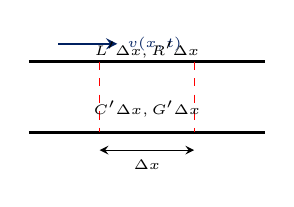
\begin{tikzpicture}[scale=0.75]
    \draw[thick] (0,1.2) -- (4.0,1.2);
    \draw[thick] (0,0) -- (4.0,0);
    \draw[dashed, red] (1.2,1.2) -- (1.2,0);
    \draw[dashed, red] (2.8,1.2) -- (2.8,0);
    \draw[<->, >=stealth] (1.2,-0.3) -- (2.8,-0.3) node[midway, below, font=\tiny] {$\Delta x$};
    \draw[->, >=stealth, thick, unibblue] (0.5,1.5) -- (1.5,1.5) node[right, font=\tiny] {$v(x,t)$};
    \node at (2.0,1.4) [font=\tiny] {$L'\Delta x, R'\Delta x$};
    \node at (2.0,0.4) [font=\tiny] {$C'\Delta x, G'\Delta x$};
  \end{tikzpicture}%
  }%
\end{minipage}\par

\vfill

% Kotak Formula Rujukan Teknis & Standar Industri
\begin{tcolorbox}[colback=unibblue!3,colframe=unibblue,colbacktitle=unibblue,coltitle=white,boxrule=0.6pt,arc=2pt,left=6pt,right=6pt,top=3pt,bottom=3pt,title=\textbf{\scriptsize FORMULA RUJUKAN TEKNIS \& STANDAR INDUSTRI TERKAIT}]
  \scriptsize
  \begin{itemize}[leftmargin=*, nosep]
  \item Persamaan Telegrafer Saluran Transmisi: $\frac{\partial v}{\partial x} = -R' i - L' \frac{\partial i}{\partial t}$, \quad $\frac{\partial i}{\partial x} = -G' v - C' \frac{\partial v}{\partial t}$
  \item Persamaan Gelombang Saluran Tanpa Rugi ($R'=G'=0$): $\frac{\partial^2 v}{\partial x^2} = L' C' \frac{\partial^2 v}{\partial t^2} = \frac{1}{v_p^2} \frac{\partial^2 v}{\partial t^2}$
  \item Parameter Karakteristik Saluran: Kecepatan Rambat $v_p = \frac{1}{\sqrt{L'C'}}$, Impedansi Karakteristik $Z_0 = \sqrt{\frac{L'}{C'}}$
  \item Koefisien Refleksi Tegangan pada Beban $Z_L$: $\Gamma_L = \frac{Z_L - Z_0}{Z_L + Z_0}$
\end{itemize}
\end{tcolorbox}

\newpage
% ==================== HALAMAN 2 ====================

\noindent{\textbf{\color{unibblue}\large BAGIAN II: ANALISIS SISTEM, EVALUASI STANDAR, \& KOMPUTASI JULIA}}\par
\vspace{1mm}

% Soal C4
\noindent\textbf{4. (C4 - Menganalisis \textbar\ Bobot: 20 Poin)}\par\vspace{0.8mm}
{\footnotesize Analisis Refleksi Gelombang Surja Petir: Saluran transmisi Soal 3 dihubungkan ke transformator daya dengan impedansi surja beban $Z_L = 1200\,\Omega$. Ketika gelombang petir beramplitudo $V_0 = 400\text{ kV}$ tiba di terminal trafo: (a) Hitung koefisien refleksi tegangan $\Gamma_L$; (b) Hitung tegangan puncak total yang dialami isolasi transformator; (c) Analisis bahaya kegagalan dielektrik akibat fenomena pantulan tegangan ini.}\par

\vspace{3.5mm}

% Soal C5
\noindent\textbf{5. (C5 - Mengevaluasi \textbar\ Bobot: 20 Poin)}\par\vspace{0.8mm}
{\footnotesize Gunakan Metode Pemisahan Variabel $v(x,t) = X(x) T(t)$ untuk memecahkan persamaan gelombang saluran tanpa rugi dengan syarat batas ujung terhubung singkat $v(0,t) = 0$ dan $v(L_s,t) = 0$. Buktikan bahwa frekuensi-frekuensi alami osilasi gelombang berdiri (*standing wave resonance*) bernilai $f_n = \frac{n v}{2 L_s}$ untuk $n = 1, 2, 3, \dots$.}\par

\vspace{3.5mm}

% Soal C6
\noindent\textbf{6. (C6 - Merancang \& Komputasi Julia \textbar\ Bobot: 15 Poin)}\par\vspace{0.8mm}
{\footnotesize Rancang program simulasi gelombang berjalan dalam bahasa \textbf{Julia} menggunakan skema beda hingga FDM (*Finite Difference Method*) untuk memvisualisasikan perambatan pulsa surja tegangan petir dari pangkal hingga memantul di ujung beban saluran transmisi. Buat animasi profil gelombang $v(x,t)$ terhadap posisi $x$.}\par

\vfill

% Tabel Rekapitulasi Skor OBE & Lembar Catatan Umpan Balik Dosen
\noindent\begin{minipage}[b]{0.62\textwidth}%
  \centering
  \scriptsize
  \begin{tabular}{|c|c|c|c|c|c|c|}
    \hline
    \rowcolor{unibblue}
    \textbf{\color{white}C1} & \textbf{\color{white}C2} & \textbf{\color{white}C3} & \textbf{\color{white}C4} & \textbf{\color{white}C5} & \textbf{\color{white}C6} & \textbf{\color{white}Total} \\
    \rowcolor{unibblue!10}
    10 Pts & 15 Pts & 20 Pts & 20 Pts & 20 Pts & 15 Pts & 100 Pts \\
    \hline
    & & & & & & \\[3mm]
    \hline
  \end{tabular}%
\end{minipage}%
\hfill%
\begin{minipage}[b]{0.35\textwidth}%
  \centering
  \scriptsize
  \textbf{Verifikasi Dosen / Asisten:}\\[6mm]
  (\dotfill)\\[1mm]
  \tiny Tanggal: \dotfill
\end{minipage}\par

\vspace{2mm}
\begin{tcolorbox}[colback=white,colframe=unibblue!40!black,colbacktitle=unibblue!10,coltitle=unibblue,boxrule=0.5pt,arc=2pt,left=5pt,right=5pt,top=3pt,bottom=3pt,title=\textbf{\tiny Catatan Evaluasi \& Umpan Balik Dosen Pengampu}]
  \tiny
  \textbf{Rubrik Pemeriksaan Pengerjaan Tugas Mandiri:}\par\vspace{0.8mm}
  $\square$ Penurunan matematis langkah-demi-langkah runtut (C1--C4) \hfill $\square$ Validasi analitis \& standar industri IEEE/IEC/SPLN akurat (C5)\\[0.8mm]
  $\square$ Skrip program Julia mandiri \& grafik visualisasi terlampir (C6) \hfill $\square$ Kerapian format laporan \& ketepatan waktu pengumpulan\\[2.0mm]
  \textbf{Catatan / Koreksi Khusus Dosen:}\\[1.6cm]
\end{tcolorbox}

\end{document}
